% ---
% Assinaturas
% ---
% Isto é um exemplo de Folha de aprovação, elemento obrigatório da NBR
% 14724/2011 (seção 4.2.1.3). Você pode utilizar este modelo até a aprovação
% do trabalho. Após isso, substitua todo o conteúdo deste arquivo por uma
% imagem da página assinada pela banca com o comando abaixo:
%
% \includepdf{folhadeaprovacao_final.pdf}
%
\begin{folhadeaprovacao}
	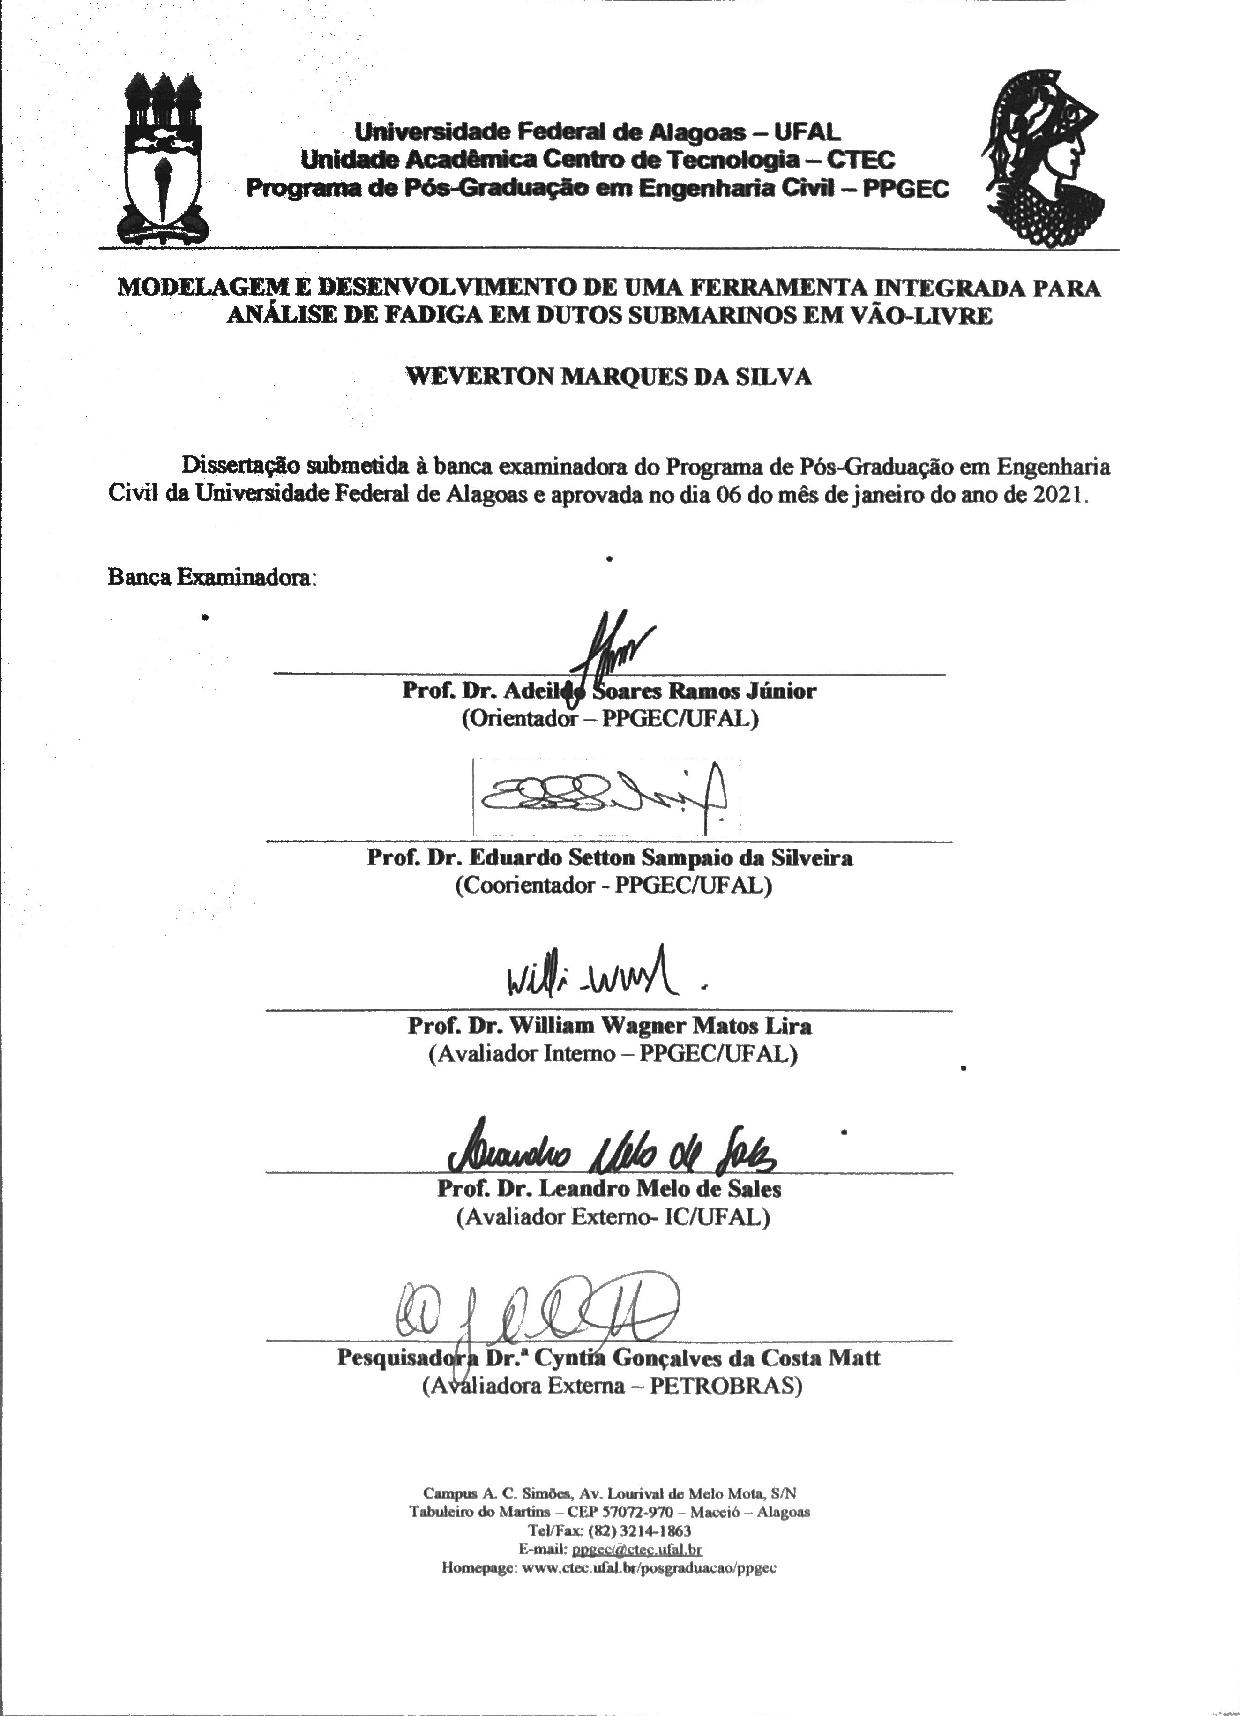
\includepdf{pretextual/folha_de_aprovacao}
	% \begin{center}
	% 	\textbf{Folha de Aprovação}
	% 	\vfill

	% 	AUTOR: \MakeUppercase{\imprimirautor}

	% 	\vfill
	% 	\imprimirtitulo
	% 	\vfill

	% 	\hspace{.45\textwidth}
	% 	\begin{minipage}{.5\textwidth}
	% 		\imprimirpreambulo
	% 	\end{minipage}%
	% 	\vfill

	% 	Trabalho aprovado. \imprimirlocal, 28 de setembro de 2016:
	% \end{center}

	% \assinatura{\textbf{\imprimirorientador} \\ Orientador}
	% \assinatura{\textbf{\imprimircoorientador} \\ Co-Orientador}
	% \assinatura{\textbf{William Wagner Matos Lira} \\ Convidado 1}
	% \assinatura{\textbf{Leandro Melo de Sales} \\ Convidado 2}

\end{folhadeaprovacao}